% Use only LaTeX2e, calling the article.cls class and 12-point type.

\documentclass[12pt]{article}

% Users of the {thebibliography} environment or BibTeX should use the
% scicite.sty package, downloadable from *Science* at
% www.sciencemag.org/about/authors/prep/TeX_help/ .
% This package should properly format in-text
% reference calls and reference-list numbers.

\usepackage{scicite}

% Use times if you have the font installed; otherwise, comment out the
% following line.

\usepackage{times}

\usepackage{graphicx}

% The preamble here sets up a lot of new/revised commands and
% environments.  It's annoying, but please do *not* try to strip these
% out into a separate .sty file (which could lead to the loss of some
% information when we convert the file to other formats).  Instead, keep
% them in the preamble of your main LaTeX source file.


% The following parameters seem to provide a reasonable page setup.

\topmargin -1.5cm
\oddsidemargin 0.0cm
\textwidth 16cm 
\textheight 23.5cm
\footskip 1.0cm

%The next command sets up an environment for the abstract to your paper.

\newenvironment{sciabstract}{%
\begin{quote} \bf}
{\end{quote}}

% If your reference list includes text notes as well as references,
% include the following line; otherwise, comment it out.

%\renewcommand\refname{References and Notes}

% The following lines set up an environment for the last note in the
% reference list, which commonly includes acknowledgments of funding,
% help, etc.  It's intended for users of BibTeX or the {thebibliography}
% environment.  Users who are hand-coding their references at the end
% using a list environment such as {enumerate} can simply add another
% item at the end, and it will be numbered automatically.

\newcounter{lastnote}
\newenvironment{scilastnote}{%
  \setcounter{lastnote}{\value{enumiv}}%
  \addtocounter{lastnote}{+1}%
  \begin{list}%
  {\arabic{lastnote}.}
  {\setlength{\leftmargin}{.22in}}
  {\setlength{\labelsep}{.5em}}
}
{\end{list}}

\title{Assignment 1} 

\author
{Filipe Pires [85122], João Alegria [85048]\\
\\
Information Retrieval\\
\normalsize{Department of Electronics, Telecommunications and Informatics}\\
\normalsize{University of Aveiro}\\
} 

\date{\today{}}

%%%%%%%%%%%%%%%%% END OF PREAMBLE %%%%%%%%%%%%%%%%

\begin{document} 

% Double-space the manuscript.

\baselineskip18pt

% Make the title.

\maketitle 

% Place your abstract within the special {sciabstract} environment.

%\begin{sciabstract}
  
%\end{sciabstract}

% In setting up this template for *Science* papers, we've used both
% the \section* command and the \paragraph* command for topical
% divisions.  Which you use will of course depend on the type of paper
% you're writing.  Review Articles tend to have displayed headings, for
% which \section* is more appropriate; Research Articles, when they have
% formal topical divisions at all, tend to signal them with bold text
% that runs into the paragraph, for which \paragraph* is the right
% choice.  Either way, use the asterisk (*) modifier, as shown, to
% suppress numbering.

\section*{Introduction}

This report aims to describe the work developed for the first assignment
of the discipline of 'Information Retrieval', explaining the overall
processing pipeline.
We include a short description of each class developed and of the respective
methods, as well as the instructions on how to run our code.

The program implemented in Python version 3 has the purpose of indexing
documents given as input in a compressed format.
This document indexer consists of a corpus reader, a tokenizer and the 
actual indexer.

Along with the description of the solution, we also answer to a few questions
proposed for the assignment \cite{assign1}.

\newpage
\section*{1. Architecture}

In order to maintain a modular architecture, we resorted to the Python library 
{\it Abstract Base Classes\/} (or simply ABC) \cite{abclib}.
This module provided us with the infrastructure for defining abstract classes
for each of our own modules.
As seen in Fig.\ref{fig:classdiagram}, the 3 base classes all derive from 
an ABC.

The choice of this form of architecture was due to several reasons: modules
allow the reduced coupling between system components, making it easy to replace
or add new ones; creating variations of the solution (as we will see on the
\texttt{Tokenizer} class) becomes far simpler and easier to manage; adopting this 
program structure also helps making the extension/adaptability of the 
program to other corpora structures easier to implement.

\begin{figure}[h!]
  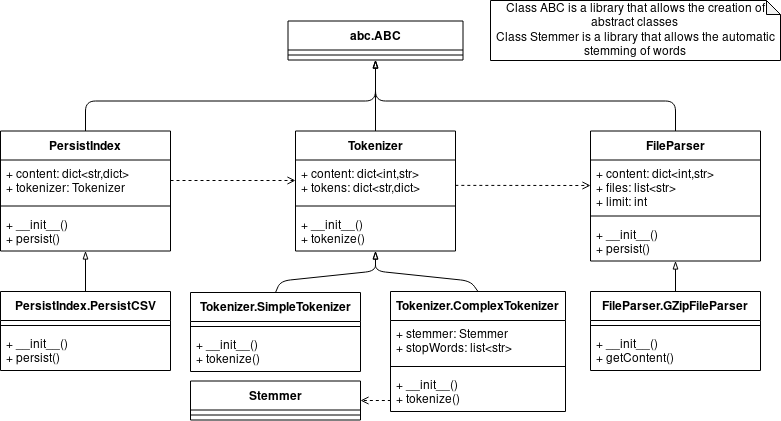
\includegraphics[width=\linewidth]{ClassDiagram.png}
  \caption{Program's class diagram.}
  \label{fig:classdiagram}
\end{figure}

The class \texttt{FileParser} is an abstract class for all file parsers.
In our case, we only needed to develop 1 derived class to parse files on
.gz format. It is \texttt{GZipFileParser} that actually ...................

\texttt{Tokenizer} is the abstract base class for our 2 Tokenizer implementations.
This class depends on the \texttt{FileParser} as it uses its ...............
The \texttt{SimpleTokenizer} contains only one method called {\it tokenize()\/} 
that replaces all non-alphabetic characters by a space, lowercases tokens, 
splits on whitespace, and ignores all tokens with less than 3 characters.
The \texttt{ComplexTokenizer}, on the other hand, is, as the name indicates, a
more complex implementation aimed to return a more valuable set of tokens.
This class integrates a stopword filter to ignore words considered not relevant
and a stemmer to standardize all words, i.e. it normalizes the terms (or tokens)
according to an algorithm that considers the English language by conflating
words with the same linguistic base form.
The stemmer used was PyStemmer \cite{pystemmer}, which is an implementation of 
Porter Stemmer, as recommended on the assignment instructions. 
For this reason, \texttt{ComplexTokenizer} depends on the class \texttt{Stemmer}.

Finally we have the \texttt{PersistIndex} abstract class.
Our implementation, \texttt{PersistCSV}, is the class responsible for persisting
the ids of the documents where a given token appears and the number of
occurrences in each of those documents, for all of the tokens from the entire
vocabulary of the input files. 
This is done by storing the data in a map structure (a Python dictionary) using
the method {\it persist()\/}.

\newpage
\section*{2. Data Flow}

The file \texttt{Indexer.py} serves as the command to be executed in order to 
indexing all documents passed as arguments.
This command has the following format:

\begin{quote}
\begin{verbatim}
$ python3 Indexer.py [-h] [-o outputFile] [-l limit] \\
  [-t tokenizer] inputFile1 [inputFile2]+
\end{verbatim}
\end{quote}

Here, \texttt{-h} is the option that presents the manual for the command usage.
Options \texttt{-o} and \texttt{-l} allow the definition of the output file's 
name and of the limit for the number of lines to be processed in each input file.
Option \texttt{-t} makes possible for the user to choose the type of tokenizer
to be used. 
The alternatives are: 'simple' for the use of the \texttt{SimpleTokenizer} class,
and 'complex' for the \texttt{ComplexTokenizer} class.
The previous arguments are all optional and the actual values for these arguments
must appear right after the respective options.
The final argument(s) of the command must be the name(s) of the input file(s) to
be indexed.

Once the arguments are validated, the program attempts to ...............

Below we present the actual implementation in Python of the function responsible 
for parsing the information source file. \\

\begingroup
\addtolength\leftmargini{-0.4in}
\addtolength\baselineskip{-0.05in}
\begin{quote}
\begin{verbatim}
 ......
\end{verbatim}
\end{quote}
\endgroup

\newpage
\section*{3. Discussion}

To test the capabilities of the developed software, we indexed 2 large 
compressed files made available along with the assignment description
with the names \texttt{2004\_TREC\_ASCII\_MEDLINE} \texttt{\_1.gz} and 
\texttt{2004\_TREC\_ASCII\_MEDLINE\_2.gz}.
Each file is a collection (corpus) of documents.
In this chapter we discuss our implementation's performance over these 
files and answer the following questions:

a) What is the total indexing time and final index size on disk?

b) What is the vocabulary size?

c) What are the ten first terms (in alphabetic order) that appear in 
only one document (document frequency = 1)?

d) What are the ten terms with highest document frequency?

To answer question a), we simple added the command \texttt{time} in the
beginning of the execution of the \texttt{Indexer.py} 
(e.g. \texttt{\$time python3 Indexer.py (...)}).
This command returned us 3 measured times during the execution, but we 
were interested only in one of them - the Elapsed real time (in seconds)
since the execution start.
After all code optimizations, the best value we could achieve was of 
\texttt{9'12''} (nine minutes and twelve seconds) and an index size on 
disk of \texttt{500.9 Mbs} with the \texttt{SimpleTokenizer} and of 
\texttt{14'15''} (fourteen minutes and fifteen seconds) and an index 
size on disk of \texttt{484.3 Mbs} with the \texttt{ComplexTokenizer}.

For the remaining questions, we developed a small script called
\texttt{IndexAnalyzer.py} that processes the output file passed as argument.
The calculated size of the vocabulary of both input files combined was of 
\texttt{N} unique terms.

The 10 first terms (ordered alphabetically) with document frequency of 1
are the following:

\begingroup
\addtolength\leftmargini{-0.4in}
\addtolength\baselineskip{-0.05in}
\begin{quote}
\begin{verbatim}
 ......
\end{verbatim}
\end{quote}
\endgroup

These were retrieved first filtering out all terms with document frequency
above 1 and then ordering the remaining alphabetically with the use of the
{\it quicksort\/} algorithm.

The 10 terms with highest document frequency are the following:

\begingroup
\addtolength\leftmargini{-0.4in}
\addtolength\baselineskip{-0.05in}
\begin{quote}
\begin{verbatim}
 ......
\end{verbatim}
\end{quote}
\endgroup

To retrieve these terms, we stored the maximum number of occurrences
during the output file's reading process and then search for the terms
with that document frequency; these terms are less than 10, we proceed 
on filtering for documents with document frequency of 1 less document
and repeat the process until the 10 terms are found.

\newpage
\section*{Conclusions}

Lorem ipsum ...

\begin{thebibliography}{9}
  \bibliographystyle{Science}

  \bibitem{assign1}
    S. Matos,
    \textit{IR: Assignment 1},
    University of Aveiro,
    2019/20.
  \bibitem{abclib}
    Abstract Base Classes,
    Python.org,
    \textit{https://docs.python.org/2/library/abc.html},
    (visited in 01/10/2019)
  \bibitem{pystemmer}
    Snowball Stem PyStemmer,
    GitHub.com,
    \textit{https://github.com/snowballstem/pystemmer},
    (visited in 01/10/2019)
  
\end{thebibliography}

\clearpage

\end{document}




















